%; whizzy paragraph -pdf xpdf -latex ./whizzypdfptex.sh
%; whizzy-paragraph "^\\\\begin{frame}"
% latex beamer presentation.
% platex, latex-beamer でコンパイルすることを想定。 

%     Tokyo Debian Meeting resources
%     Copyright (C) 2009 Junichi Uekawa
%     Copyright (C) 2009 Nobuhiro Iwamatsu

%     This program is free software; you can redistribute it and/or modify
%     it under the terms of the GNU General Public License as published by
%     the Free Software Foundation; either version 2 of the License, or
%     (at your option) any later version.

%     This program is distributed in the hope that it will be useful,
%     but WITHOUT ANY WARRANTY; without even the implied warreanty of
%     MERCHANTABILITY or FITNESS FOR A PARTICULAR PURPOSE.  See the
%     GNU General Public License for more details.

%     You should have received a copy of the GNU General Public License
%     along with this program; if not, write to the Free Software
%     Foundation, Inc., 51 Franklin St, Fifth Floor, Boston, MA  02110-1301 USA

\documentclass[cjk,dvipdfmx,12pt]{beamer}
\usetheme{Tokyo}
\usepackage{monthlypresentation}

\setbeamertemplate{footline}{\hskip1mm\insertshortdate\hfill\hbox{\insertpagenumber /\insertdocumentendpage }\hspace*{1mm}\vskip1mm}

%  preview (shell-command (concat "evince " (replace-regexp-in-string "tex$" "pdf"(buffer-file-name)) "&")) 
%  presentation (shell-command (concat "xpdf -fullscreen " (replace-regexp-in-string "tex$" "pdf"(buffer-file-name)) "&"))
%  presentation (shell-command (concat "evince " (replace-regexp-in-string "tex$" "pdf"(buffer-file-name)) "&"))

%http://www.naney.org/diki/dk/hyperref.html
%日本語EUC系環境の時
\AtBeginDvi{\special{pdf:tounicode EUC-UCS2}}
%シフトJIS系環境の時
%\AtBeginDvi{\special{pdf:tounicode 90ms-RKSJ-UCS2}}

\newenvironment{commandlinesmall}%
{\VerbatimEnvironment
  \begin{Sbox}\begin{minipage}{1.0\hsize}\begin{fontsize}{8}{8} \begin{BVerbatim}}%
{\end{BVerbatim}\end{fontsize}\end{minipage}\end{Sbox}
  \setlength{\fboxsep}{8pt}
% start on a new paragraph

\vspace{6pt}% skip before
\fcolorbox{dancerdarkblue}{dancerlightblue}{\TheSbox}

\vspace{6pt}% skip after
}
%end of commandlinesmall


\title{waylandを動かす}
\author{野島 貴英 nozzy@debian.or.jp}
\date{2013年11月16日}
\logo{
\includegraphics[width=8cm]{image200607/openlogo-light.eps}}

\begin{document}

\frame{\titlepage{}}

%\section{}

\begin{frame}{wayland! weston!}
\begin{itemize}
\item wayland\\
ディスプレイサーバーのプロトコルの一つ。
\item weston\\
 waylandプロトコルを扱えるディスプレイサーバーの実装。
\end{itemize}

 両者共にKristian H\o{}gsbergさんらが中心で鋭意開発中。

\end{frame}

\begin{frame}{wayland! weston!}
\center{\LARGE 要はウィンドウシステムの1つの実装です。}
\end{frame}

\begin{frame}{weston動いている様子(カスタマイズ無し)}
\begin{center}
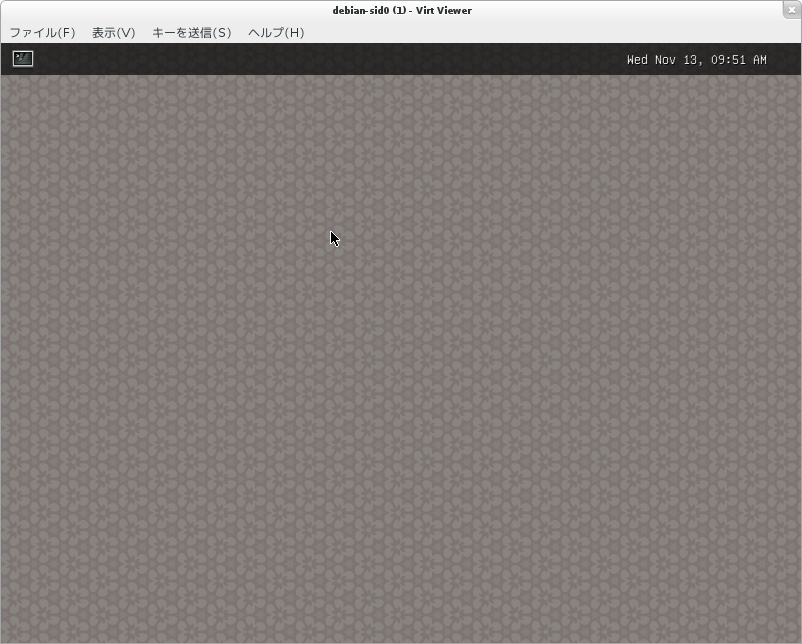
\includegraphics[width=0.8\hsize]{image201311/weston-1st-launch.png}
\end{center}
\end{frame}

\begin{frame}{weston動いている様子(weston.iniいじる)}
\begin{center}
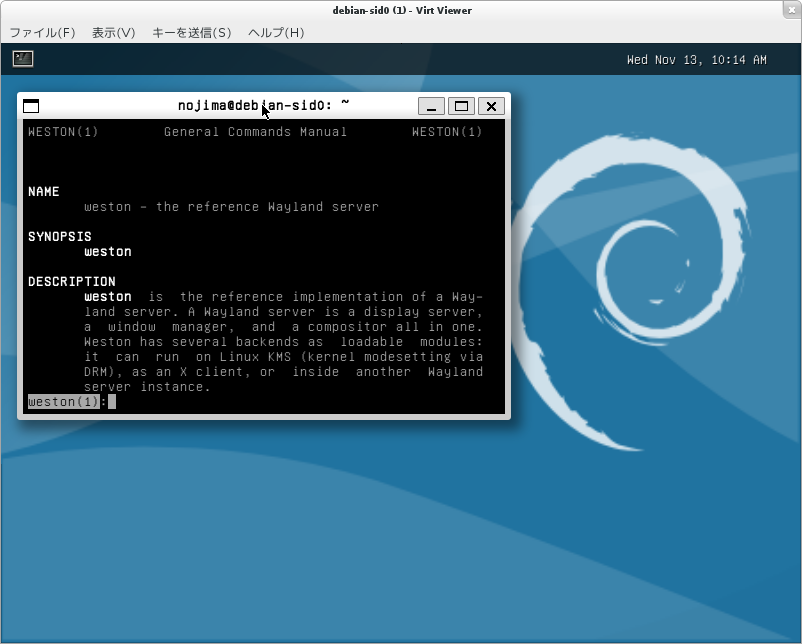
\includegraphics[width=0.8\hsize]{image201311/weston-2nd-launch.png}
\end{center}
\center{静止画だとわかりにくいのですが、にゅっとウィンドウが開いてます。      }
\end{frame}

\begin{frame}{当然の疑問:Xは?ねえ?Xは?}

 UNIX界で標準的ディスプレイサーバーの実装とプロトコルにXがあります。
が、1984年からすっごい頑張って機能拡張と保守が続けられてきたのですが、
結果的に
\begin{itemize}

\item Daniel Stone,``The real story behind Wayland and X'',linux.conf.au 2013,\\
\url{http://people.freedesktop.org/~daniels/lca2013-wayland-x11.pdf}\\
\url{http://www.youtube.com/watch?v=RIctzAQOe44}
\end{itemize}
で説明があるとおりで、もういろいろ無理出まくってる状況なので、一回やり直した方がいいんじゃね?という状況になっているようです。

\end{frame}


\begin{frame}{当然の疑問:Xは?ねえ?Xは?}

補足:\\
waylandについてphoronixの記事\footnote{http://www.phoronix.com}にて、H\o{}gsbergさんによれば、「チラついたり描画してるところが見えちゃったりする事の無いウィンドウシステムを作る」(``every frame is perfect'')ということですが、実際にはXの諸々の問題をどうにかする(見直す)という事も含んでいるようです。

\end{frame}


\begin{frame}{weston出力デバイスは何がつかえる?}
upstreamが用意している出力デバイスと、debian sid提供のwestonの利用できる出力デバイス一覧。
\begin{table}[ht]
\begin{center}
\small
\begin{tabular}{|l|l|l|l|l|}
\hline 
項番&出力デバイス&バックエンド名&パッケージ搭載済\\
\hline \hline
1& DRM/KMS & drm-backend.so & ○ \\
2& フレームバッファ & fbdev-backend.so & ○ \\
3& X & x11-backend.so & ○ \\
4& Wayland & wayland-backend.so & ○ \\
5& Headless & headless-backend.so & ○ \\
5& Rassberry Pi & rpi-backend.so & × \\
6& RDP & rdp-backend.so & × \\
\hline
\end{tabular}
\end{center}
\end{table}

\end{frame}

\begin{frame}[containsverbatim]{動かす時の前準備}

\begin{enumerate}
\item まずは、apt-get install westonしてね!
\item 環境変数XDG\_RUNNTIME\_DIRに読み書き可能なディレクトリを指定。\\
\begin{itemize}
\item systemdが動く場合:systemd-logindが勝手に指定してくれるよ!
\item systemdが動かない場合:export XDG\_RUNNTIME\_DIR=/tmpとかすればOK
\end{itemize}
\item weston-launchコマンドを使うなら、/etc/groupのweston-launchグループにユーザを追加。\\
\begin{commandline}
# usermod -a -G weston-launch <your-login-id>
...この後ログアウトして、ログインしなおしてね...
\end{commandline}
\end{enumerate}
\begin{center}
以上!
\end{center}
\end{frame}

\begin{frame}[containsverbatim]{X上で動かす}
\begin{commandline}
Xのターミナルから
$ weston 
\end{commandline}
%$
\begin{center}
!一番簡単!
\end{center}
\end{frame}

\begin{frame}{DRM/KMS上で動かす}

 linuxのカーネルのモジュールのうち、ウィンドウシステムでよくつかわれる物に、DRM/KMSがあります。

\begin{description}
\item [DRM] Direct Rendering Managerの略。グラフィクカードを複数のアプリケーションから扱う時に必要な機能や、そもそもアプリケーションがグラフィックカードを扱うのに必要な機能(DMA転送のコントロールとか、リソースロックとか、Memory Mapped I/Oを直接いじる時に安全にいじれるようにするとか)を提供するモジュール。
\end{description}

 要は、ウィンドウシステム上で3Dとかやろうとすると、アプリもウィンドウシステムもみんなよってたかってGPUをいじらなきゃいけないので、誰か調停しないといけない。これを行う実装がDRM。次から次へと出てくるGPUの仕様に振り回されてる状況。


\end{frame}

\begin{frame}{DRM/KMS上で動かす}

\begin{description}
\item [KMS] Kernel-based Mode Settingの略。グラフィックカードを初期化するのに、グラフィックカードを初期化するコードをユーザランドに置いて行うと、テキストモードとグラフィクスモードへの移行の度に画面がバチバチ揺らぐ現象が起きる。カーネル側でブート時にあらかじめグラフィクスモードへ移行させておき、ユーザランドからはカーネルが設定したグラフィクスモードをそのまま使えるようにすれば、グラフィックを扱うアプリが起動する度にバチバチ画面が揺らぐのを抑える事ができる。この処理を実現するモジュール。
\end{description}

\end{frame}

\begin{frame}[containsverbatim]{DRM/KMS上でweston動かす}

 DRM/KMS上でweston動かすなら、

\begin{enumerate}
\item グラフィカルなログイン画面が出ているようであれば、こちらを停止させます。\\
例:gdm3が立ち上がっている場合の止め方
\begin{commandline}
Ctrl-Alt-F1等を押下してコンソールに切り替える
$ su
# service gdm3 stop
\end{commandline}
%$
\item KMS/DRMドライバが有効であることを確かめます。
\begin{commandline}
$ lsmod | egrep '(i915|radeon|nouveau)'
...(i915/radeon/nouveauのどれかの文字列が出ればOK)...
\end{commandline}
%$
\item 最後にwestonを動かします。
\begin{commandline}
$ weston-launch
\end{commandline}
%$
\end{enumerate}
\end{frame}

\begin{frame}{DRM/KMSのデモ}

\begin{itemize}
\item デモってみます。
\item こちらはIntelのチップセット入りのSONY VAIOのマシンですが、DRM/KMSで動かすと外部VGA端子にもwestonの画面が立ち上がってますので、デモに便利です。カーソルは画面左端へ持っていけばそのまま外部VGA端子に出力されている画面に移動します。
\end{itemize}

\end{frame}

\begin{frame}{フレームバッファで動かす}

 Linuxには昔からフレームバッファデバイスというのがあります。こちらを使う事により、
コンソールに対して2Dグラフィクス描画ができます。こちらを利用してwestonを動かします。なお、詳しい動かし方は第106回東京エリアDebian勉強会資料を参照ください。

 \begin{itemize}
 \item KVMで、Xの力を借りずにwestonを動かすにはこちらが便利です。
 \item debian sidのパッケージはweston-1.3.0ですが、fbdev-backend.soに仮想端末制御まわりのバグがあり、正常に動作しません。ですので、勉強会資料に記載したとおり、weston-1.3.1のパッケージを作り導入して稼働させる必要があります。
 \end{itemize}

\end{frame}

\begin{frame}[containsverbatim]{おまけ:waylandで動かす}

 westonはwayland-backend.soを使う事により、weston上でwestonを動かす事が出来ます。

 \begin{enumerate}
 \item westonを今までの方法で動かす
 \item wayland-terminalを開き、新しいソケットを指定して、westonを動かす。
\begin{commandline}
$ weston -Swayland-1 --width=640 --height=400
(width/heightを指定しないと画面からはみ出すので)
\end{commandline}
%$
 \end{enumerate}

\center{Xnestみたいなもんです}

\end{frame}

\begin{frame}{おまけ:waylandで動かす}

\begin{center}
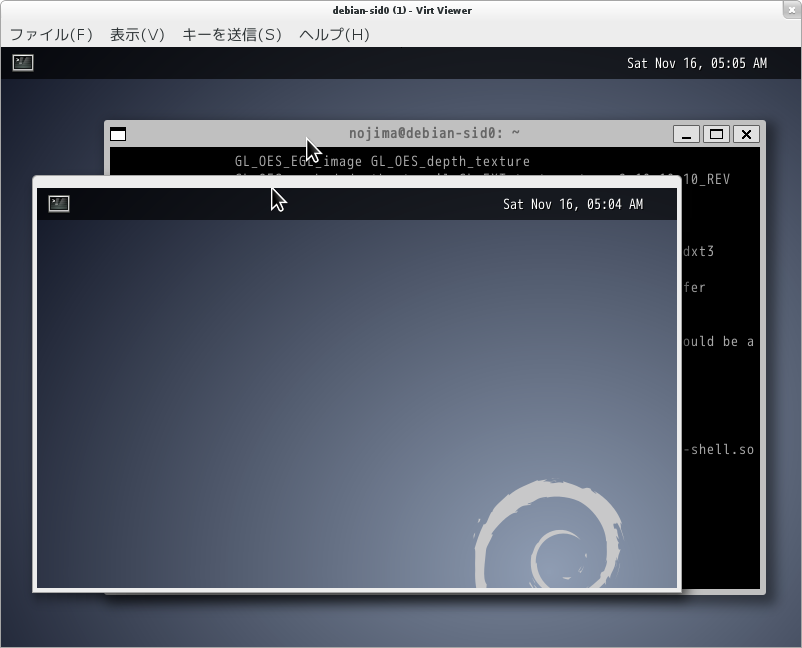
\includegraphics[width=0.8\hsize]{image201311/weston-wayland-launch.png}
\end{center}

\end{frame}


\begin{frame}{debianでのwaylandまわり対応状況}

debianでのwayland/westonまわり対応状況は次の通りです。

\begin{itemize}
\item weston上でXアプリケーションを動かす為の機能である、XWaylandは、現在のdebian sidでも動作しません。なので、未だXアプリケーションをそのままweston上で動かす事ができません。\\
理由: Xサーバーにwayland用のパッチが当たっていない状況です。ですので、xwayland.soがXを起動する際に指定する-waylandというオプションを現行のdebianのXが知らないため、すぐにXが落ちてしまいます。\\
10月にdebian-x@d.oにパッチが流れていた\footnote{\url{http://lists.debian.org/debian-x/2013/10/msg00205.html}}ので、きっとそのうち搭載される?かも。
\end{itemize}

\end{frame}

\begin{frame}[containsverbatim]{debianでのwaylandまわり対応状況}

\begin{itemize}
\item debian sidで提供されるgtkなどの有名どころのツールキットも、debian提供のパッケージではwaylandが有効になっていないため、westonの上で動かす事ができません。
\end{itemize}

本来なら、
\begin{commandline}
$ aptitude install gtk-3-examples
$ env GDK_BACKEND=wayland gtk3-demo
\end{commandline}
とかすれば、gtkのデモがweston/wayland上で動くはずなんですけどね...

\end{frame}

\begin{frame}{westonとwaylandアプリの構造}

\begin{center}
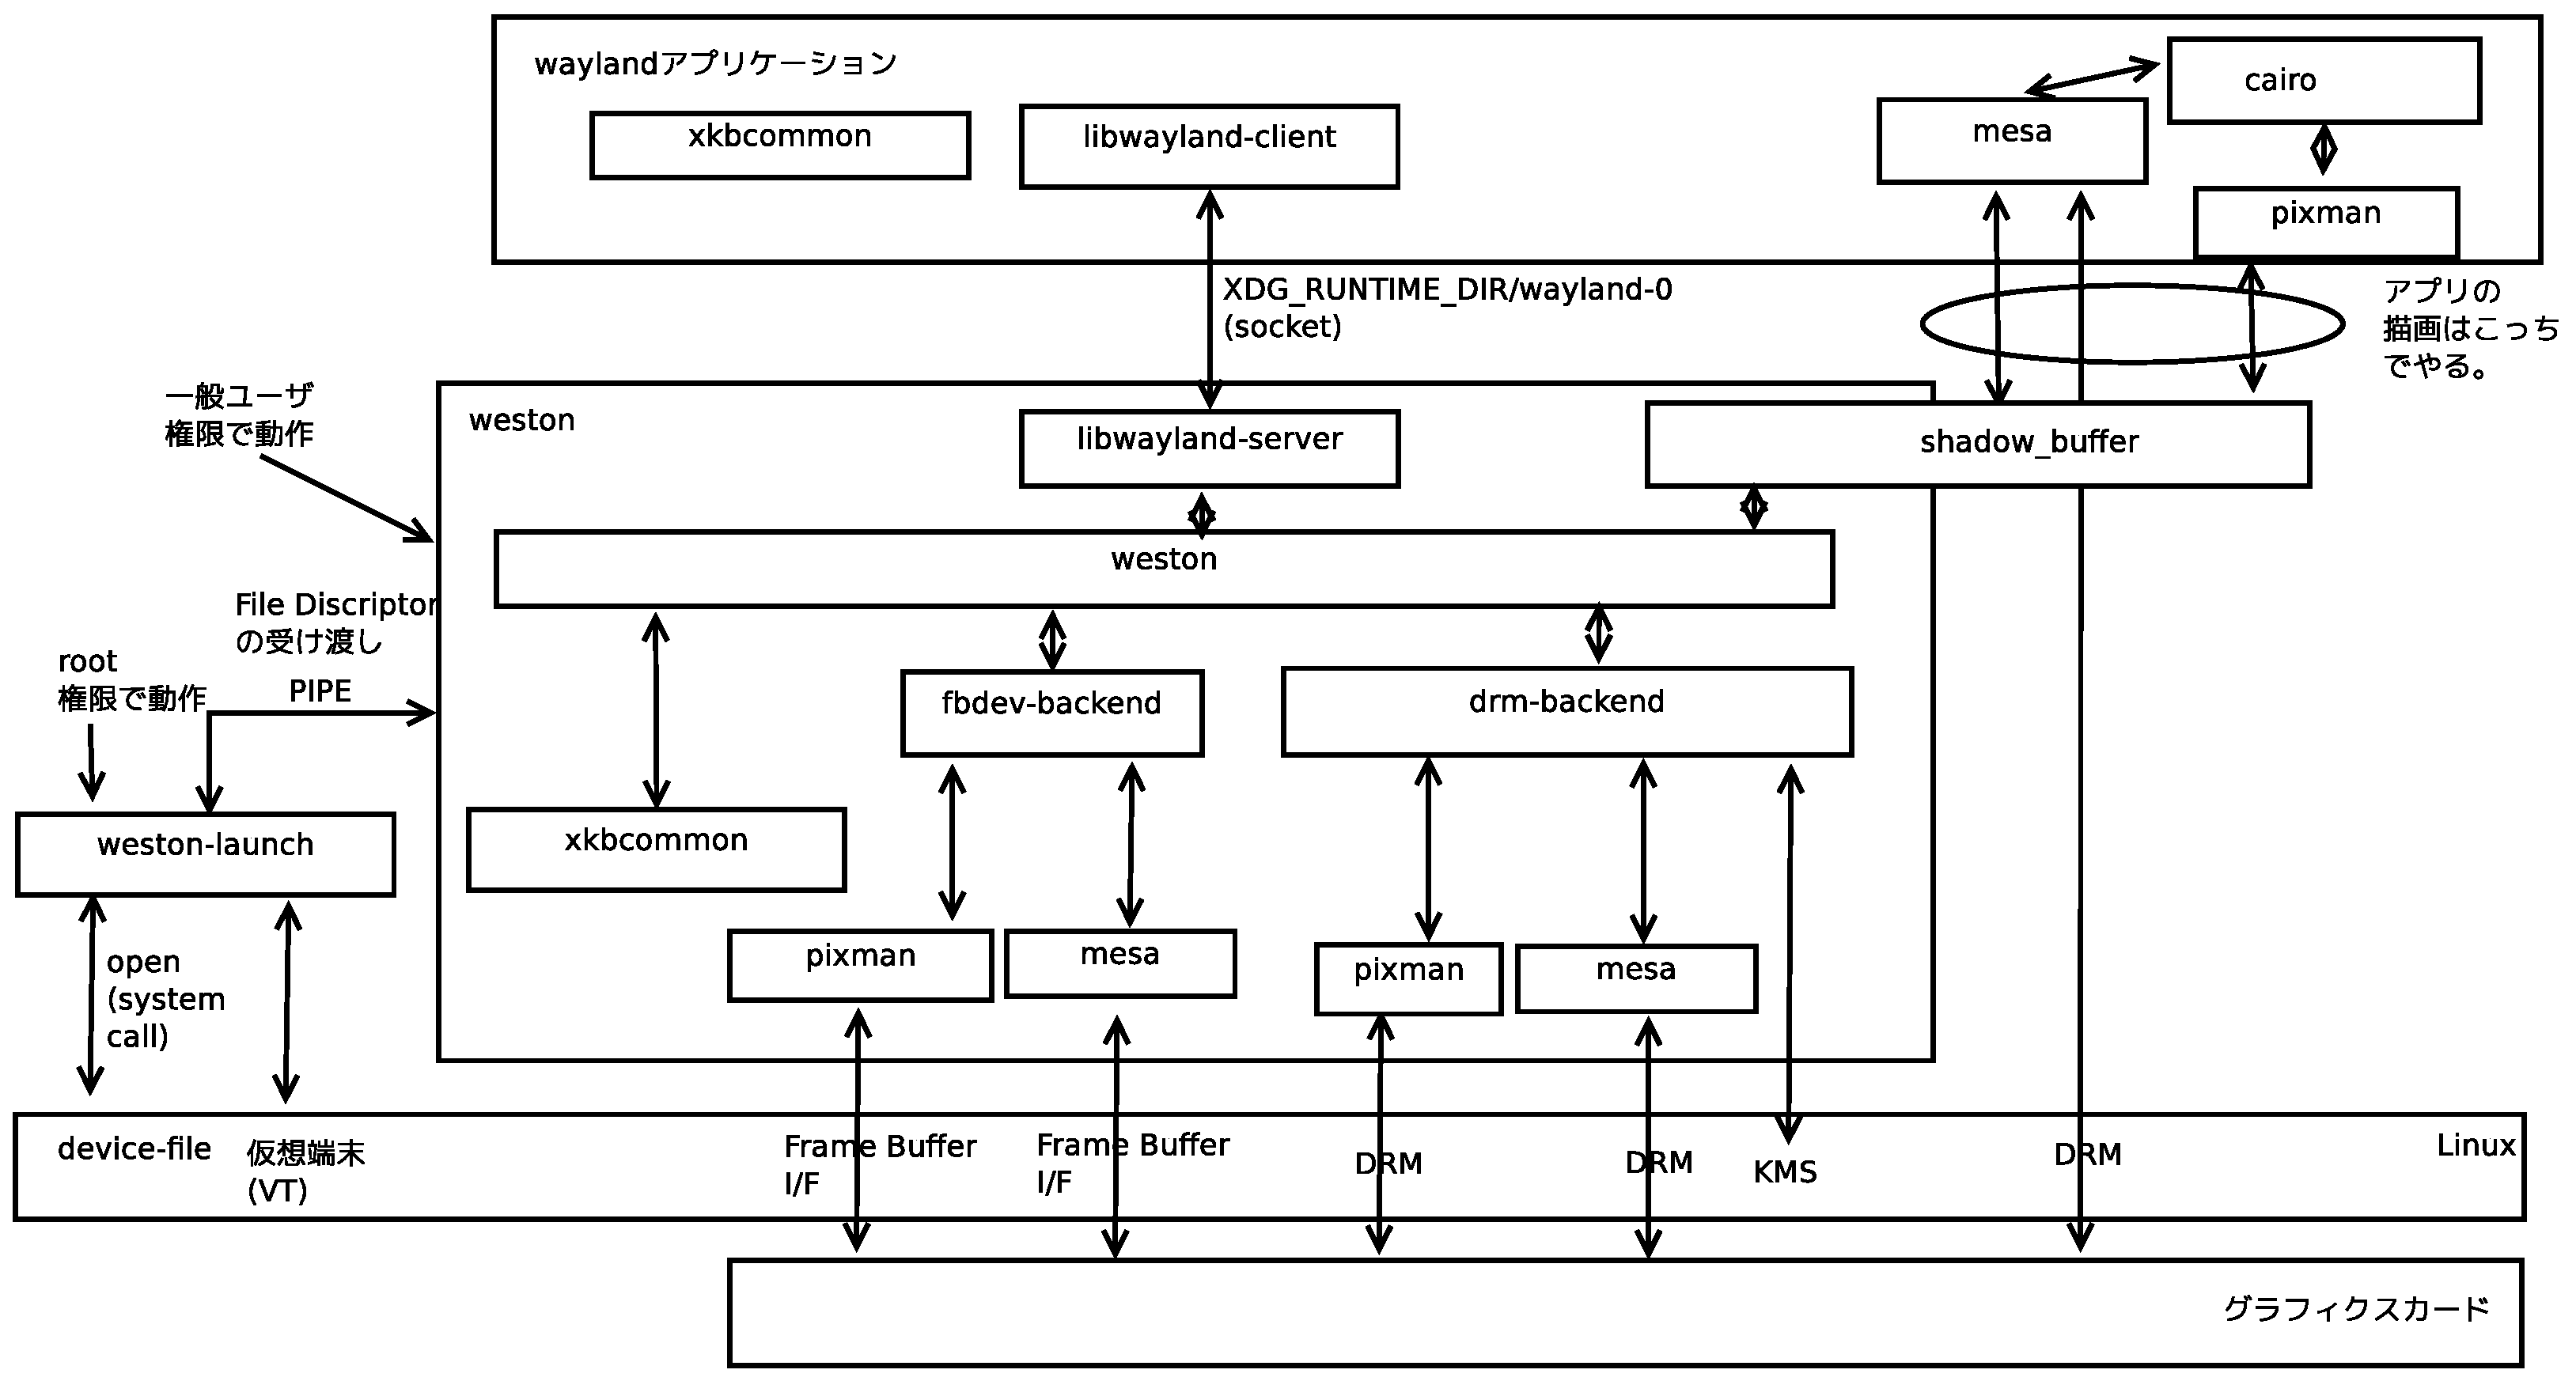
\includegraphics[width=0.95\hsize]{image201311/wayland-internal-schema.eps}
\end{center}

\begin{center}
とっても単純!
\end{center}

\end{frame}

\begin{frame}{westonとwaylandアプリの構造}

みての通り、

\begin{itemize}
\item Xで実現されているレベルのネットワーク透過性は、もう設計上完全に省略(投げ捨ててるとも言える)
\item 代わりに、レイヤ(pixmap)/サーフェース(EGL/mesa)を活用しまくって、エレガントにウインドウシステムを実現してます。ウインドウをレイヤ、もしくは、サーフェースの上に描く構造にして、westonの指示により一気に全画面を合成する作りになってます(コンポジット型。)なので、書き換えの際のチラつきがなく、また、ウィンドウの透過も正しい透過の描画が可能です
(後ろのウィンドウが正しい重ね合わせで透ける等。)
\item 入力デバイス対応は、xkbcommonとかを活用しています。
\end{itemize}

\end{frame}

\begin{frame}{westonとwaylandアプリの構造}

\begin{itemize}
\item weston-launchはsuidでroot権限での動作をします。weston-launchはweston稼働中にroot権限がどうしても必要な操作を担当し、root権限不要になった資源(ファイルディスクリプタ等)を、socket経由で一般ユーザ権限で動くwestonへ引き渡しています(sendmsg/recvmsgの方法ですね)
\end{itemize}

\end{frame}

\begin{frame}{westonとwaylandアプリの構造}
どうやって描画してるの?
\begin{center}
\includegraphics[width=0.6\hsize]{image201311/wayland-composite-explain.eps}
\end{center}
\end{frame}

\begin{frame}[containsverbatim]{westonが動くDRM/KMSの状況}

\begin{itemize}
\item 今のところ、\verb+$(MESA_SRC)/include/pci_ids/pci_id_driver_map.h+中の\verb+driver_map+変数に定義されているチップセットはmesaにより3Dアクセラレーション付きで対応しているようです(自分はi915のみ評価。)※求む!radion/nouveauでの動作評価。
\end{itemize}

\end{frame}

\begin{frame}[containsverbatim]{westonが動くDRM/KMSの状況}
mesaに含まれているGPUドライバの例(GPUじゃないのもあるけど...)
\begin{commandlinesmall}
$(MESA_SRC)/include/pci_ids/pci_id_driver_map.h
の
 static const struct {
 61    int vendor_id;
 62    const char *driver;
 63    const int *chip_ids;
 64    int num_chips_ids;
 65 } driver_map[] = {
 66    { 0x8086, "i915", i915_chip_ids, ARRAY_SIZE(i915_chip_ids) },
 67    { 0x8086, "i965", i965_chip_ids, ARRAY_SIZE(i965_chip_ids) },
 68 #ifndef DRIVER_MAP_GALLIUM_ONLY
 69    { 0x1002, "radeon", r100_chip_ids, ARRAY_SIZE(r100_chip_ids) },
 70    { 0x1002, "r200", r200_chip_ids, ARRAY_SIZE(r200_chip_ids) },
 71 #endif
 72    { 0x1002, "r300", r300_chip_ids, ARRAY_SIZE(r300_chip_ids) },
 73    { 0x1002, "r600", r600_chip_ids, ARRAY_SIZE(r600_chip_ids) },
 74    { 0x1002, "radeonsi", radeonsi_chip_ids, ARRAY_SIZE(radeonsi_chip_ids) },
 75    { 0x10de, "nouveau", NULL, -1 },
 76    { 0x15ad, "vmwgfx", vmwgfx_chip_ids, ARRAY_SIZE(vmwgfx_chip_ids) },
 77    { 0x0000, NULL, NULL, 0 },
 78 };
\end{commandlinesmall}
%$
\end{frame}

\begin{frame}[containsverbatim]{westonが動くDRM/KMSの状況}

\begin{itemize}
\item '--use-pixman'を付与してweston-launchを起動してGPUによる3Dアクセラレーションを投げ捨てれば、\verb+/lib/modules/`uname -r`/kernel/drivers/gpu/drm/+ 以下にあるDRM/KMSドライバを利用してmesaが対応していないGPUの元でも動かすことができそうなものですが、何故かwestonがSEGVで落ちまくるなどの現象が発生するようです。こちらの理由は、自分には良く解っていません。\\
(これがなければ、グラフィクスチップの2Dアクセラレーションすら無いフレームバッファーは使わなくても済む...)
\end{itemize}

\end{frame}

\begin{frame}{その他周辺技術}
 
 linux向けのグラフィクス界隈は、いろいろ技術がありまして...よい文章は↓

\begin{center}
DRM/KMS,FB,V4L2の説明でよい文章↓\\
\url{http://elinux.org/images/2/22/KMS_FB_and_V4L2_How_to_Select_a_Graphics_and_Video_API.pdf}
\end{center}

\end{frame}

\begin{frame}{その他周辺技術}

\begin{description}
\item [pixman] pixmanは、2Dの描画をアセンブラで記述する等して、非常に最適化された2D描画を可能にするライブラリです。画像の合成、ポリゴンを台形単位に分割して描画する機能なども持ちます。アンチエイリアシングなども搭載しているため非常に美しい描画が可能です。しかしながら、使い方のドキュメントが存在してないのが残念です。本家:\url{http://www.pixman.org/}
\end{description}

\end{frame}

\begin{frame}{その他周辺技術}

\begin{description}
\item [mesa] mesaは、オープンソースでの実装のOpenGLです。最近のトレンドとしては、
gallium3dとllvmpipeがあります。gallium3dはstate trackerと呼ばれる仕組みを用いて、GPU個別の事情をうまく住み分ける事ができるアーキテクチャであり、llvmpipeはCPUのソフトウェアレンダラの実装ですが、LLVMの技術を利用して高速化とシェーダ言語への対応を行っているものです。本家:\url{http://www.mesa3d.com}
\end{description}

gallium3dの良い文献↓\\
Gallium3D Mesa's New Driver Model\\
\url{http://www.slideshare.net/olvaffe/gallium3d-mesas-new-driver-model}
\end{frame}



\begin{frame}{情報源}

 オープンソースのグラフィクス事情について詳しい情報が活発に載るニュースサイトは、
\begin{quote}
phoronix\\
\url{http://www.phoronix.com}
\end{quote}
があります。ここは、毎日オープンソースプロダクトのグラフィクス事情についての記事が精力的に書かれ、weston/waylandの動向もこちらに真っ先に乗ります。オープンソースプロダクトのグラフィクス性能は独自のベンチマーク評価を実際に行い公表しているのも面白いです。

もし、オープンソースのグラフィクス事情を素早くキャッチしたい時はこちらのサイトがおすすめです。他にも良いサイトがあったら教えて〜!
\end{frame}

\begin{frame}{おわりに}

 weston/waylandは、いろいろ賑わってきていますし、実装もシンプルでやることはいろいろと多いと思ってます。ですので、Hackするにはちょうどよいプロダクトだとおもいます。


\end{frame}

\end{document}

;;; Local Variables: ***
;;; outline-regexp: "\\([ 	]*\\\\\\(documentstyle\\|documentclass\\|emtext\\|section\\|begin{frame}\\)\\*?[ 	]*[[{]\\|[]+\\)" ***
;;; End: ***
